\documentclass[../thesis.tex]{subfiles}

\begin{document}

  \chapter{Experimental}
  \label{ch:experimental}

    \section{Membrane production}
    \label{sec:membrane-production}

      The alumina membrane production process starts with a circular wafer of amorphous aluminum of $\SI{99,999}{\percent}$ purity and $\SI{1}{\milli\meter}$ thickness. In a first anodizing step, parallel pores are created that show a hexagonal order (\cref{subsec:anodizing}). Then, the remaining aluminum of the wafer is dissolved by immersion in an acid as specified in \cref{eq:aluminum-dis-acid} in \cref{subsec:al-dissolution}. Next, the so called \textit{barrier layer} closing the pores on the bottom end is etched by floating the wafer on oxalic acid (\cref{subsec:barrier-layer-dissolution}). Last, the pore diameters are reduced using atomic layer deposition (ALD).

      With an initial diameter of $d_\mathrm{wafer}=\SI{5}{\centi\meter}$, one wafer is broken into twelve square membranes, the side length being $l_\mathrm{membrane}=\SI{1}{\centi\meter}$. Since the wafer has a thickness of $l_\mathrm{pore}=\SI{30}{\micro\meter}$ to $\SI{60}{\micro\meter}$, the wafer is precut using a scallpell before the anodization. This step enables to cleave the wafer easily. As the cleaving step is performed at the very end of the membrane synthesis, the suqare membranes are expected to show equivalent characteristics.


      \subsection{Anodizing}
      \label{subsec:anodizing}

          \Cref{fig:anodizing} shows a sketch of the anodizing setup. The bulk aluminum wafer (compare \cref{fig:bulk-al}), which functions as the anode, is glued to a copper plate using conductive silver paste. The copper plate is then covered by non conductive polymer CAF4 leaving only the circular surface of the wafer expozed to the acid. A platinum plate that is placed at a horizontal distance of $\SI{3}{\centi\meter}$ from the anode functions as cathode. The whole setup is immersed in oxalic acid that is continuously stirred. The anodization is conducted at a constant voltage $U_\mathrm{anodizing}$.

          \subfile{tikz/membrane_production/anodizing.tex}

          The pore diameter $d_\mathrm{pore}$ and the inter pore distance $d_\mathrm{interpore}$ depend on the anodizing conditions. Along with $U_\mathrm{anodizing}$, these are given by the oxalic acid's molar concentration $n_\mathrm{\ce{C2H2O4}}$ and its acid temperature $T_\mathrm{\ce{C2H2O4}}$. Their variation changes the pore diameters between  $\SI{10}{\nano\meter}$ and $\SI{100}{\nano\meter}$. To produce wafers with the pore specifications
          \begin{align*}
            \begin{split}
              d_\mathrm{pore}=\SI{40}{\nano\meter},    \\
              d_\mathrm{interpore}=\SI{100}{\nano\meter},
            \end{split}
          \end{align*}
          the anodization is conducted using the parameters
          \begin{align*}
            \begin{split}
              U_\mathrm{anodizing}^{\SI{40}{\nano\meter}} &= \SI{40}{\volt}, \\
              n_\mathrm{\ce{C2H2O4}} &= \SI{0,5}{\mol\per\litre},  \\
              T_\mathrm{\ce{C2H2O4}} &= \SI{15}{\celsius}.
            \end{split}
            \label{eq:anodizing-parameters}
          \end{align*}
          This makes for a growth rate of alumina of
          \begin{equation*}
            r_{\ce{Al2O3}} \approx \SI{8}{\micro\meter\per\second}.
          \end{equation*}
          To ensure that parallel pores are produced, a two step anodization procedure is followed.
          \medskip

          The first anodizing treats the raw bulk aluminum wafer. By the oxalic acid \ce{C2H2O4}, pathways are etched into the aluminum which follow no pattern at first. Only some of them continue to grow forming real pores, though. With the ongoing anodizing, pores start to combine to form larger pores and finally areas of hexagonally arrange pores are created throughout the wafer. The longer the anodizing process is carried out, the wider these ordered areas become. Figure \cref{fig:first-anodizing} shows the cross-section of a wafer observable at this point. Because the process transforms aluminum to alumina at a given penetration speed, the so called \textit{barrier layer} of alumina separates the pores from the bulk aluminum.
          \medskip

          Before the second anodizing, the wafer is immersed in a mixture of chromic and phosphoric acid with the concentrations
          \begin{align*}
            \begin{split}
              n_\mathrm{\ce{H3PO4}} &= \SI{0,4}{\mol\per\litre}    \\
              n_\mathrm{\ce{CrO3}} &= \SI{0,2}{\mol\per\litre}
            \end{split}
          \end{align*}
          at a temperature of
          \begin{equation*}
            T_\mathrm{\ce{CrO3}}^\mathrm{\ce{H3PO4}}=\SI{0,2}{\mol\per\litre}.
          \end{equation*}
          Hereby the created alumina is dissolved yielding a slightly thinner wafer of bulk aluminum, where the thickness $d_\mathrm{Al}'$ depends on the time of the first anodizing. The relevant difference to the initial wafer are the areas of hexagonally arranged hollows (compare figure \cref{fig:al-dissolution-1}).

          Due to this new surface structure, the second anodizing yields a wafer with a top layer of alumina penetrated by parallel, hexagonally arranged pores. Again, the \textit{barrier layer} of alumina separates the pores from the bulk aluminum as illustrated in figure \cref{fig:second-anodizing}. Increasing the time of the second anodizing increases the length of the pores $l_\mathrm{pore}$ and hereby the thickness of the final wafer. As the second anodizing is carried out  under the same conditions as the first, the pore size $d_\mathrm{pore}$ is the same in both production steps.


          \subfile{tikz/membrane_production/production_stages.tex}


      \subsection{Aluminum dissolution}
      \label{subsec:al-dissolution}

        To dissolve the remaining aluminum on the bottom side of the wafer, it is immersed in an acid composed of
        \begin{equation}
          \SI{27,2}{\gram}\quad\ce{CuCl2} + \SI{0,2}{\l}\quad\ce{HCL}(\SI{37}{\percent}) + \SI{0,8}{\l}\quad\ce{H2O}
          \label{eq:aluminum-dis-acid}
        \end{equation}
        at a temperature of
        \begin{equation}
          T = \SI{0}{\celsius}
        \end{equation}
        as shown in figure \cref{fig:al-dissolution-setup}. The latter transforms the aluminum to copper in a very exothermic reaction. A lot of turbulences are created and thus this step limits either the thickness or the size of the wafers because they can easily break.

        \subfile{tikz/membrane_production/aluminum_dissolution.tex}


      \subsection{Barrier layer dissolution}
      \label{subsec:barrier-layer-dissolution}

          The \textit{barrier layer} dissolution is done using phosphoric acid of the concentration
          \begin{equation}
              n_\mathrm{\ce{H3O4P}} = \SI{0,2}{\mol\per\l}.
          \end{equation}
          To dissolve the \textit{barrier layer} and hereby open the pores, the wafers are floated on phosphoric acid as shown in figure \cref{fig:float}. After $\SI{15}{\minute}$ to $\SI{30}{\minute}$, the wafer starts showing milky aspects (compare \cref{fig:milky-aspects-photo}). This is due to opening pores which fill with acid before others as will be explained in more detail in \cref{sec:opening-problem}. The phenomenom lasts for about
          \begin{equation}
            t_\mathrm{milky}=\SI{3}{\minute}
          \end{equation}
          before they disappear and the wafer becomes transparent again. From this point, the new wafers (295 and 296 with more to come) are floated for $\SI{15}{\minute}$ more to ensure well open pores (in contrast to bad open pores, which will be discussed in \cref{subsec:bad-open-pores}). Just before removing the wafers from the phosphoric acid, a liquid film covers their whole surface as photographed in \cref{fig:filmed-membrane-photo}.

          \begin{figure}[p]
            \centering
            \subfloat[]{
            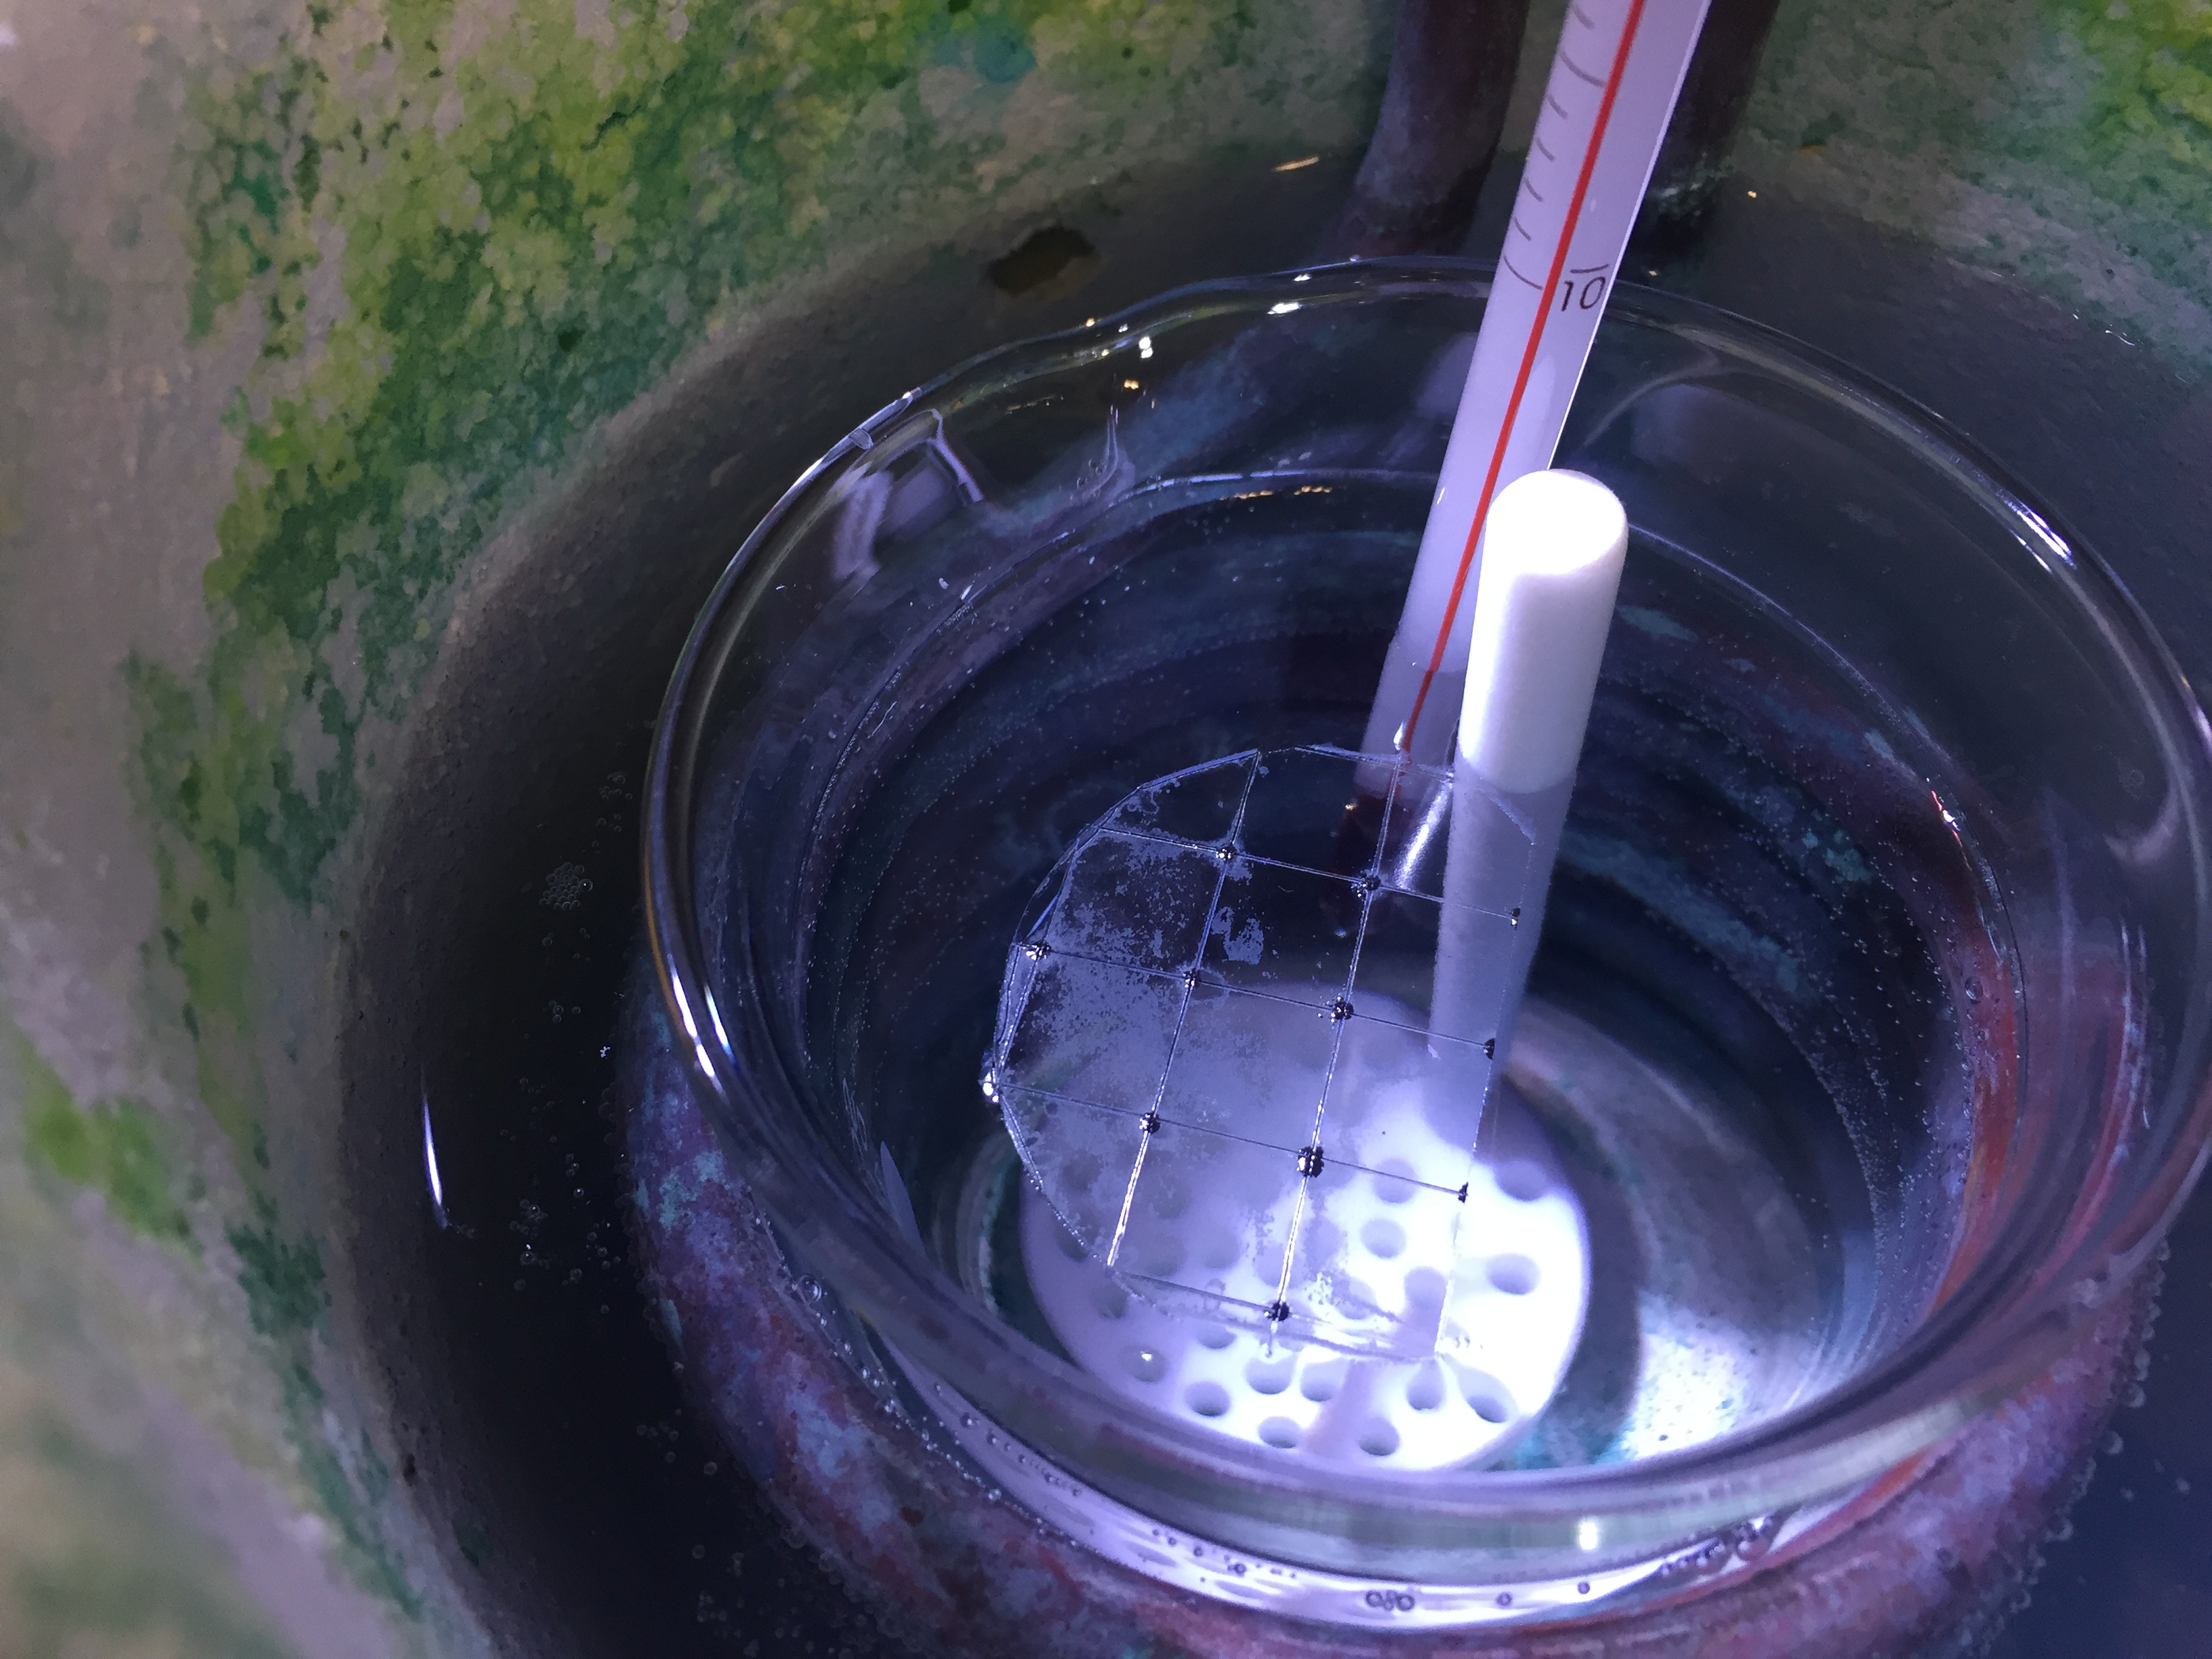
\includegraphics[width=0.9\textwidth]{images/milky_aspects.JPG}
            \label{fig:milky-aspects-photo}}\\
            \subfloat[]{
            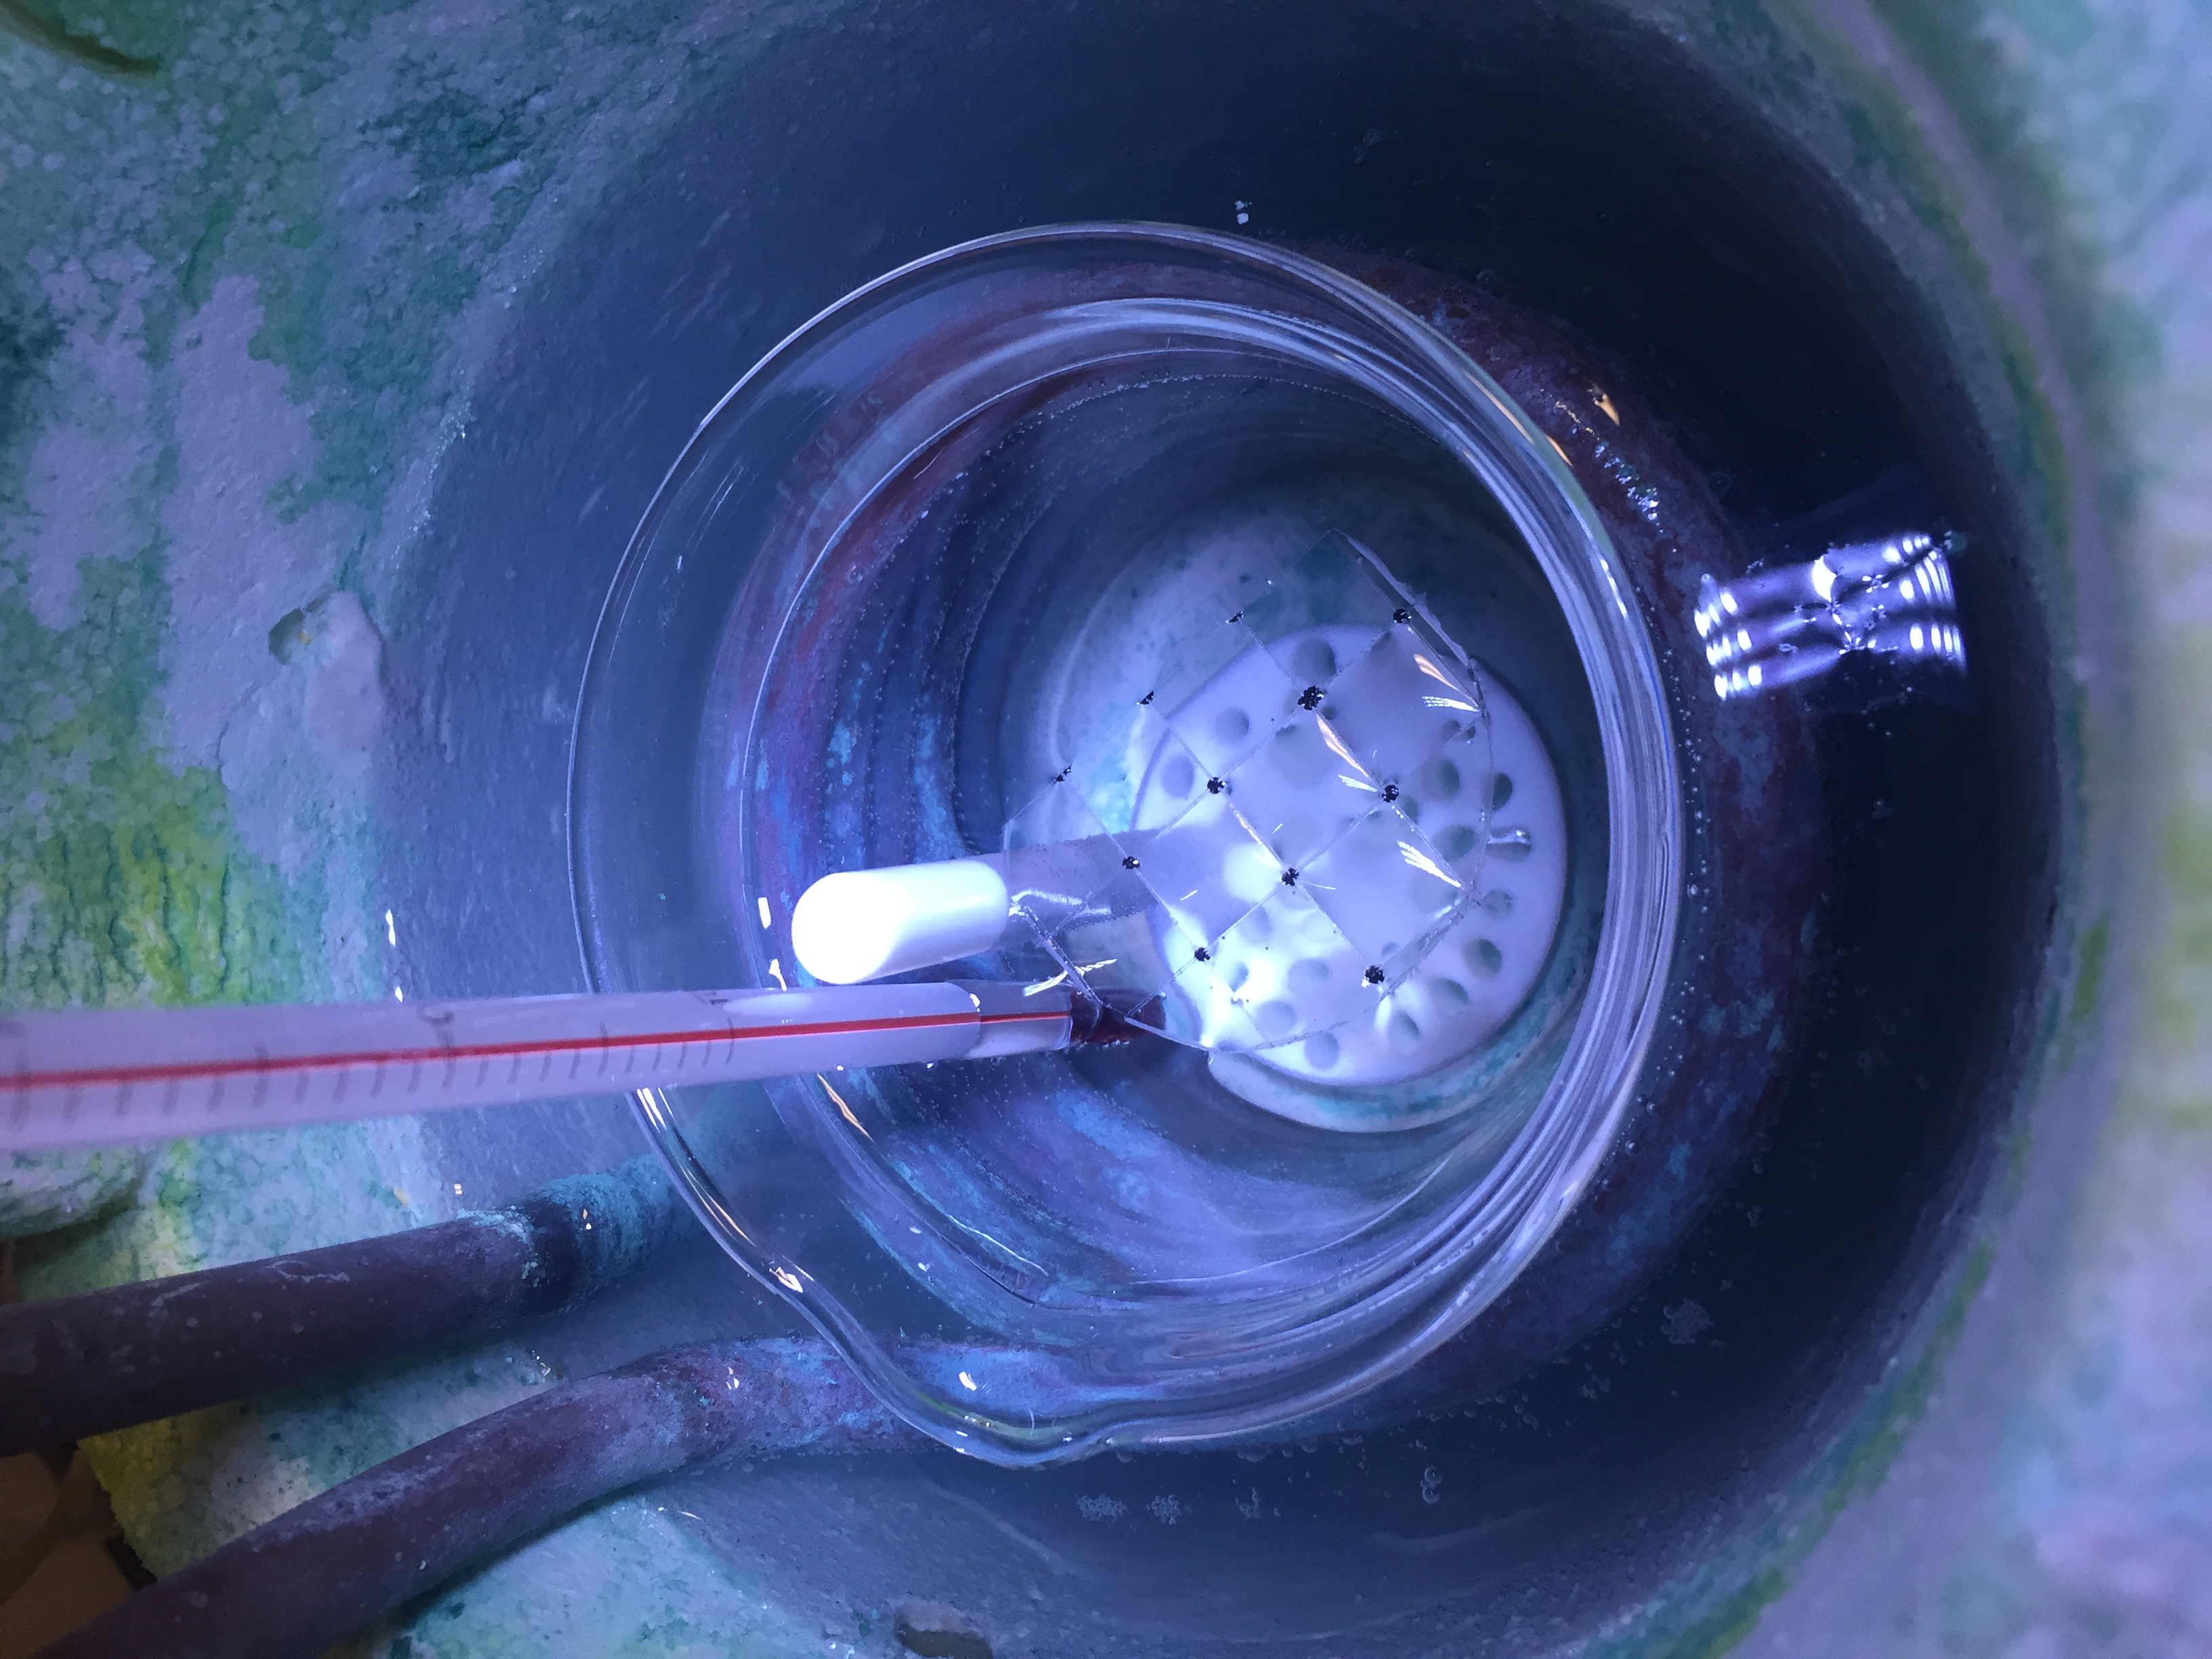
\includegraphics[width=0.9\textwidth]{images/filmed_membrane.JPG}
            \label{fig:filmed-membrane-photo}}
            \caption{Photos taken during the \textit{barrier layer} dissolution step. \protect\subref{fig:milky-aspects-photo} shows the milky aspects that appear during the floating of the wafers. In \protect\subref{fig:filmed-membrane-photo}, a film of phosphoric acid covers the whole wafer at the end of the process.}
            \label{fig:barrier-layer-dissolution-photos}
          \end{figure}

      \subsection{Atomic layer deposition}
      \label{subsec:ald}

        \subfile{tikz/ald/ald_plane.tex}

        Atomic layer deposition (ALD) is a thin film deposition method. \Cref{fig:ald} illustrates the following explications. Within a reaction chamber, the substrate is expozed to a first precursor (red in \cref{fig:ald-1}). This precursor coats the substrate with a monolayer of molecules in a self limited reaction. When the whole substrate is covered, no reactive sites remain and therefore no more molecules are deposited. Upon evacuation of the reaction chamber, the monolayer remains on the substrate (compare \cref{fig:ald-2}), which is then expozed to a second precursor (\cref{fig:ald-3}). Like the first one, this second precursor covers the substrate's surface with a monolayer of molecules (\cref{fig:ald-4}). This process is repeated until the desired thickness of deposition on the substrate has been reached (\cref{fig:ald-5} and \protect\subref{fig:ald-6}). Fundamental for the ALD process is that the two precursors are reactants.
        \medskip

        For the ALD on the alumina membranes the reaction chamber is heated to
        \begin{equation*}
          T_\mathrm{reaction-chamber}=\SI{200}{\celsius}.
        \end{equation*}
        The used precursors are trimethylaluminium (TMA) and water. This makes for an expected growth rate of
        \begin{equation*}
          g_\mathrm{ALD}=\SI{1,1}{\angstrom}
        \end{equation*}
        per cycle (\cite{SalPoi:ALD}). Since in this experiment the ALD process is used to reduce the pore diameters of the pores, the expected reduction rate of the pores is
        \begin{equation*}
          \delta d_\mathrm{pore}=\SI{2,2}{\angstrom}.
        \end{equation*}


      \subsection{Terminology}

        In the course of this article, the term \textit{solution side} refers to the surface of the membranes that has been anodized according to \cref{subsec:anodizing}. The \textit{aluminum side} is the opposite side of the membranes that is still covered by aluminum after the anodization procedure. Furthermore, the \textit{top end of a pore} is on the \textit{solution side}, wheras the \textit{bottom end of a pore} corresponds to the \textit{aluminum side}.


  \section{Scanning electron microscopy}
  \label{sec:sem}

    Scanning electron microiscopy (SEM) is used to characterize the nanoporous alumina membranes. While the measurements are very fast in comparison to the isotherm measurements, SEM is destructive and yields the pore diameters with limited precision.

    To start with, as alumina is a non conductive material, a conductor must be deposited on the membranes' surfaces. In \textit{Institut Néel}, gold is used to this end. This process does not only reduce the diameters of the pores, but also destroys the membranes. The slight constriction the gold forms at the end of the pores changes the isotherms and moreover, the membranes are not transparent to red light anymore, which prevents further transmission measurements.

    Generally, the SEM only records images of the membranes' surfaces. Since the pores' length is three orders larger in magnitude than than the pores' diameter, the aquired information does not serve for a precise characterisation of the pores' shapes.


    Moreover, the porosity of the membranes is not known and thus, the threshhold of the binarisation of the images that is done in the course of the diameter extraction. In conclusion, the measured pore diameters are rather uncertain.
    \medskip


    \subsection{Statisical evaluation of the SEM images}

      In the course of the internship, I programmed a statistical anlysis of the SEM images with the possibility to either use the mean gray intensity or a manual set threshhold for the image binarisation. From the binary files, the largest inscribed circle is computed for every pore. This data is then plotted on a histogram that also evaluates the circularity of the pores. The largest inscribed circle is used because the liquid film tends to form a circular meniscus within the pore due to the stresses implied by different meniscus curvatures (compare \textsc{Laplace-Young} quation). These results are then to be compared to the diameters derived from the condensation and evaporation models.


  \section{Experimental setup}
  \label{sec:experimental-setup}

    The experimental setup consists of two independent parts. To record isotherms, the core of the experiment is the volumetric measurement conducted in the setup explained in \cref{subsec:volumetric-setup}. In addition to that, there are a light transmission setup and a camera setup that can be set up one at a time. Both setups are used to monitor what happens during the absorption and desorption isotherms using optics. While the camera setup accumulates data for the whole surface of the membrane, the light transmission measurement probes a small area of the membrane. Both methods are used to measure the heterogenities of the processes of condensation and evaporation and to put them in context with the volumetric isotherms. The advantage of the laser transmission measurement is the ease of the data evaluation.


    \subsection{Volumetric setup}
    \label{subsec:volumetric-setup}

        The initial volumetric setup is sketched in \cref{fig:setup}. A reservoir of liquid hexane immersed in a thermostatted bath (\textsc{Lauda}) at a controlled temperature $T_\mathrm{bath}$ acts as a source of hexane gas. The dependency of the vapor pressure $P_\mathrm{v}$ ob the bath's temperature $T_\mathrm{bath}$ is given by \textsc{Antoine} equation
        \begin{equation}
          P_\mathrm{v}=10^{A- \frac{B}{C+T_\mathrm{bath}}},
          \label{eq:antoine-equation}
        \end{equation}
        which is plotted for hexane in the relevant temperature range in \cref{fig:antoine} using the \textsc{Antoine} equation parameters
        \begin{align}
          \begin{split}
              A=4,00266,	\\
              B=1171,53,  \\
              C=-48.784
          \end{split}
          \label{eq:antoine-parameters} %https://webbook.nist.gov/cgi/cbook.cgi?ID=C110543&Mask=4&Type=ANTOINE&Plot=on#ANTOINE
        \end{align}

        \subfile{tikz/temperature_pressure/temp_p.tex}

        (\cite{antoine-pars}). This reservoir is connected to the rest of the experiment by a valve. Behind the valve lies a cross leading to a pressure gauge $P_\mathrm{res}$, via another valve to a primary pump (void), and via a \textsc{Pfeiffer} EVR116 needle microvalve to the cell containing the sample membrane. This branch is also connected to a pressure gauge $P_\mathrm{cell}$. The microvalve is the key part of the experiment as it allows for the extremely low flow rates that are necessary for the conducted experiment (\cref{sec:experimental-procedure}). Furthermore, the temperature of the cell and that of the thermostatted bath are monitored by the thermometers $T_\mathrm{cell}$ and $T_\mathrm{res}$.
        \medskip

        \subfile{tikz/setup/setup.tex}

        The whole experiment setup is placed in a climatized room set to \begin{equation}
            T_\mathrm{room} = \SI{23}{\celsius}.
        \end{equation}
        The coldest point of the experiment must be the cell containing the sample membrane as to be sure no hexane condenses anywhere else in the setup. Therefore, the temperature of the cell is regulated to
        \begin{equation}
            T_\mathrm{cell} = \SI{19}{\celsius}
        \end{equation}
        as mentioned in \cref{subsec:tcell-regulation}. The the reservoir of bulk hexane is set to a temperature of
        \begin{equation}
            T_\mathrm{res} = \SI{21}{\celsius}
        \end{equation}
        using the \textsc{Lauda} allowing to fully condense the cell at $T_\mathrm{cell}$.


        \subsubsection{Cell temperature regulation}
        \label{subsec:tcell-regulation}

          The cell itself is made of a copper ring which is sealed on both siwhiledes using sapphire windows. Making use of indium O-rings, the windows are pressed onto the copper ring by two stainless steel rings. This circular cell is designed so it can be inserted in a copper clamp which is connected to a \textsc{Peltier} heat pump and a heater. Moreover, two thermometers are installed - one for the temperature regulation feedback loop and one for the output value. While the power of the \textsc{Peltier} is fixed, the heater's power output is controlled by the feedback loop. From the microvalve to the pressure gauge $P_\mathrm{cell}$, the setup is packed in styrofoam for thermal insulation from the room temperature and also to minimize the gradient inside this part of the setup. At first, the regulation has been run via a regular computer. As this led to breakdowns of the regulation for short periods of time multiple times per hour,  the regulation was then externalized to a \textsc{raspberry pi}. It regulates the temperature to $T_\mathrm{cell}=\SI{19.000(5)}{\celsius}$.


        \subsubsection{Pressure gauges}

            Because of its high resolution, a \textsc{Keller} pressure gauge was used for $P_\mathrm{cell}$ at first. My first experiments revealed that its construction contains a porous O'ring that could be identified as the source of degassing inside the system. After discussions with the retailers, we chose to swap the pressure gauge for a \textsc{Wika} S10 which exposes only metallic parts to the hexane. $P_\mathrm{res}$ uses the same model of pressure gauge.


        \subsection{Laser transmission setup}
        \label{subsec:laser_transmission_setup}

          The laser transmission setup is sketched out in \cref{fig:laser_transmission_setup}. In the path of the initial laser beam, a collimator and a diaphragm are placed before the cell. After being scattered by the membrane, the beam then passes another diaphragm and a collecting lense before hitting the photodiode.

          \subfile{tikz/setup/laser_transmission_setup.tex}


        \subsection{Camera setup}
        \label{subsec:camera-setup}

          To record images of the membranes during the absoprtion and desorption isotherms, a camera is installed and focused on the alumina membrane. A green LED lamp by \textsc{Thor Labs} is used as a light source. The camera and the light source are positioned on opposite sides of the membrane as to measure the transmission. For the setup, a \textsc{Zyla} camera by \textsc{Andor} is used with a $\SI{50}{\milli\meter}$ makro lens.


  \section{Experimental procedure}
  \label{sec:experimental-procedure}
 Only one of the two is set in place at the same time though
    To start an experiment (here also referred to as an isotherm) the valve $U_1$ is closed while $U_2$ and the \textsc{Pfeiffer} microvalve $U_\mathrm{PV}$ are fully opened. This allows the primary pump, which experimentally realizes the void, to pump the system. After setup has been assembled, the first pumping process serves to clean the system from the air that unavoidably enters the system when placing a membrane inside the cell (or removing it from the cell). After this, the air that enters the system through leaks is pumped in between two isotherm measurements. To start an isotherm after a pumping process, $U_2$ is closed and the condensation process initialized by setting $U_\mathrm{PV}$ to a sufficiently low opening voltage and opening $U_1$. Sufficiently low opening voltage shall imply that the condensation plateau of the condensation inside the membrane's pores is distinguishable on the recorded $P$ over $t$ isotherm. The employed flow rate's magnitude is  $\SI{e-5}{\milli\bar\litre\per\second}$.

    To also record the bulk condensation plateau, which defines the saturated vapor pressure $P_\mathrm{sv}$ in the evaluation process, the setup is left condensing iniside the cell for five hours after the pressure inside the cell reaches $P_\mathrm{cell} = \SI{150}{\milli\bar}$. This way a small amount of bulk liquid is condensed inside the cell. At the end of the process, all the valves are closed.

    The evaporation process is then initialized by opening the valve $U_2$. Meanwhile, the \textsc{Pfeiffer} microvalve is set to a sufficiently low opening voltage $U_\mathrm{PV}$ to permit the primary pump to pump the system. Again, sufficiently low implies that the evaporation plateau of the  liquid evaporating from the membrane's pores is visible on the recorded $P$ over $t$ isotherm. The system is left in this state till the pressure inside the cell $P_\mathrm{cell}$ reached a given setpoint at which the microvalve is fully opened to pump the system and prepare for another isotherm.


    \subsection{Bypass}
    \label{subsec:bypass}

        As the flow rate of hexane in the system depends on the opening of the \textsc{Pfeiffer} microvalve and the pressures $P_\mathrm{res}$ and $P_\mathrm{cell}$, this opening should always be the same to be able to compare multiple isotherms. As my experiments raised the suspicion of a hysteresis upon opening and closing of the microvalve, a bypass is added to the setup. \Cref{fig:setup-bypass} shows the new setup, which allows to pump the part of the system containing the cell without changing the opening of the \textsc{Pfeiffer} microvalve. This way there is no need to ever change the before and one potential error source is removed from the system.
        \medskip

        \subfile{tikz/setup/setup_bypass.tex}


        The green volume of the system, which is the one of interest for the isotherm computation, is calibrated using \textsc{Boyle}'s law. Its volume is approximately
        \begin{equation}
            V_\mathrm{cell}=\SI{8,3}{\centi\meter\cubic}.
        \end{equation}


    \subsubsection{Changing the membrane}
    \label{sssec:changing-the-sample}

        To change the sample, the copper cell must be opened and therefore detached from the rest of the system. After placing the membrane to be measured inside the cell, the latter is reconnected to the system. As a result, the inside of the cell is at atmospheric pressure. Before the bypass was installed, to pump the cell, the \textsc{Pfeiffer} microvalve had to be opened. Using the small opening also used for the isotherms would have made for an unbearably long pumping process. For an approximation please refer to \cref{subfig:vs_time} in \cref{subsec:volumetric-computation} where hexane is pumped from the system. As the evaluation of the volumetric measurements depends strongly on the opening of the \textsc{Pfeiffer} microvalve which is not guaranteed to reopen without a hysteresis even if the same voltage as before is applied, the bypass has been installed to create a way to pump the system without touching the \textsc{Pfeiffer}'s opening. From this point on, the contamination of the cell with degasing grease and the VCR connectors, that leak a small amount of air into the system, are the most prominent hazards of the membrane changing process.



  \section{Isotherm computation}
  \label{sec:isotherm-computation}

    In the following, evaluation of the recorded raw data is presented for volumetric (\cref{subsec:volumetric-computation}) and for the optical measurements (\cref{subsec:optical-computation}).


    \subsection{Volumetric isotherm}
    \label{subsec:volumetric-computation}


      The volumetric isotherms are obtained through a calibration of the \textsc{Pfeiffer} needle microvalve. \Cref{subfig:vs_time} shows the pressure inside the cell versus time for one measurement without membrane and one with membrane inside the cell. When there is no membrane inside the cell, there is only one bulk condensation and evaporation plateau visible on the curve. In contrast to that, additional condensation and evaporation plateaus appear when there is a membrane inside the cell. These additional plateaus correspond to the dips on the so called \textit{pressure loop} plot displayed in \cref{subfig:vs_pressure}. From here on, the following indices shall be used:
      \begin{align*}
          \begin{split}
              &1 \longrightarrow \textrm{no membrane} \\
              &2 \longrightarrow \textrm{membrane}.
              \label{eq:index_assignments}
          \end{split}
      \end{align*}
      Furthermore, the variables $P_i$, $\dot{P}_i$, $V_i$, $T_i$, $n_i$ and $\dot{n}_i$, $i\in \{1,2\}$, refer to the values measured inside of the cell, in explanation the red marked part of the system in \cref{fig:setup-bypass}. The raw isotherms of the two experiments are shown in \cref{fig:raw-isotherms}. The plateaus of the yellow curve with membrane inside the cell of the plot versus time  correspond to the dips of the time derivative of the pressure of the versus pressure plot. This can be explained by the hexane condensing inside the membrane's pores at a given pressure due to which the continuing matter flow into the cell does not yield an increase of pressure.
      \medskip

      \subfile{tikz/graphs/295b_membrane_vs_nomembrane/295b_membrane_vs_nomembrane.tex}

      Regarding the system with and empty cell, the ideal gas law is used to compute the flow rate of hexane. The content of the cell without membrane inside the cell is given by
      \begin{equation*}
          n_1 = \frac{P_1V_1}{RT_1},
      \end{equation*}
      taking into account that the temperature of the cell is regulated at $T_1$ and the volume $V_1$ is constant, the flow of matter is
      \begin{equation*}
          \dot{n}_1 = \frac{V_1}{RT_1}\cdot \dot{P}_1.
          \label{eq:n1}
      \end{equation*}
      For the system with a membrane inside the cell the flow of matter is the sum of the flow into the membrane $\dot{n}_2^\mathrm{mem}$ and the flow into the system volume excluding the membrane $\dot{n}_2^\mathrm{cell}$. This can be rewritten yielding
      \begin{equation*}
          \dot{n}_2^\mathrm{mem} = \dot{n}_2 - \dot{n}_2^\mathrm{cell},
      \end{equation*}
      where $\dot{n}^\mathrm{cell}_2$ is given by the ideal gas law. Using the fact that the flow through the \textsc{Pfeiffer} valve only depends on the pressures $P_i^\mathrm{tank}$ and $P_i^\mathrm{cell}$, assuming that $P_1^\mathrm{tank} = P_2^\mathrm{tank}$ leads to
      \begin{align}
          \begin{split}
              \dot{n}_2^\mathrm{mem}(P_2) &= \dot{n}_1(P_2) - \dot{n}_2^\mathrm{cell}(P_2)\\
              &=\frac{V_1}{RT_1}\cdot \dot{P}_1(P_2) - \frac{V_2}{RT_2}\cdot \dot{P}_2(P_2)
          \end{split}
          \label{eq:ndot-membrane}
      \end{align}
      \Cref{fig:iso-computation} shows the computation steps visually using the respective plots versus time.

      \subfile{tikz/graphs/295d_integration_visualization/295d_integration_visualization.tex}

      As the temperature of the system is regulated ($T = T_1 = T_2 = \mathrm{const.}$) and because $V = V_1 \approx V_2$ since $V_\mathrm{mem} \ll V_1$, equation \cref{eq:ndot-membrane} yields
      \begin{equation*}
          n_2^\mathrm{membrane} = \frac{V}{RT}\int_0^{t_2}\left(\dot{P}_1(t_1') - \dot{P}_2(t_2')\right) \mathrm{d}t_2',
          \label{eq:nmembrane-1}
      \end{equation*}
      with $t_1'$ such that
      \begin{equation*}
        P_1(t_1')=P_2(t_2').
      \end{equation*}
      Important at this point is the dependency of $\dot{P}_1(t_1)$ on $t_1$ while the integration is over $t_2$.

      As the experimental setup yields discreet values at given time intervals $\Delta t$, the data evaluation makes use of a sum rather than an integration.
      \begin{equation}
          n = \frac{V}{RT} \sum \left( \dot{P}_1 ( P_1 = P_2) - \dot{P}_2(P_2) \right) \cdot \Delta t
          \label{eq:nmembrane}
      \end{equation}
      yields the molar amount of hexane condensed inside the membrane. Figure \cref{fig:iso} shows the result of the integration \cref{eq:nmembrane} for membrane 296d. It is a absorption and desorption isotherm for hexane inside the porous alumina membrane. The bulk condensation and evaporation is not visible, as it is also recorded with the reference isotherm without membrane inside the cell.

      What strikes the eye is the sharp rise of the condensation branch that does not start at the liquid fraction $LF=0$. The same goes for the evaporation branch. It only drops to a liquid fraction value $LF>0$ and then decreases superimposed with the condensation branch. The reason for this initial rise of the isotherms could be to be due to the build up of a film on the membranes surfaces due to the attraction by the pores' walls. This is part of the theory of condensation and evaporation in confinement even though the film is ignored in the basic \textsc{Kelvin} equation (\cref{sec:kelvin-equation}).
      \medskip

      The pressure inside the cell $P_\mathrm{cell}$ can be translated to pore diameters $d_\mathrm{pore}^\mathrm{Kelvin}$ using the \textsc{Kelvin} equations \cref{eq:p-eq} and \cref{eq:p-sp}. As this computation is just a model that needs to be tested for small pore diameters, oftentimes the isotherms are plotted on a relative pressure
      \begin{equation*}
        P_\mathrm{rel}=\frac{P_\mathrm{v}}{P_\mathrm{sv}}.
      \end{equation*}
      Furthermore, to simplify the comparison of isotherms measured for different membranes, the condensed amount of hexane $n$ is converted to the liquid fraction $LF$ by deviding by the maximum value of $n$ for most of the displayed isotherms.

      For the computation of the introduced physical sizes, the saturated vapor pressure $P_\mathrm{sv}$ must be determined.


      \subsubsection{Porosity}
      \label{sssec:porosity}

        As explained in \cref{sec:sem}, knowing the porosity of the membranes allows to do a more precise analysis of the SEM images. To this end, the porosity of the membranes is computed from the molar amount of matter of hexane condensed within the membranes' pores (\cref{eq:nmembrane}). Furthermore, for the pressure range $\SI{0}{\milli\bar}$ to $\SI{160}{\milli\bar}$, hexane in its liquid form can be regarded as incompressible and therefore the hexane's volume be computed via
        \begin{equation*}
            V_\mathrm{hex} = n_\mathrm{hex} \cdot V_\mathrm{mol, hex}.
        \end{equation*}.
        The thickness $l_\mathrm{pore}$ of the membranes is determined by SEM images. This works sufficiently precise since the magnitude of the membranes' thickness is micrometers and the contrast between the carbon tape and the membrane itself is very sharp. Finally, the area $A_\mathrm{membrane}$ of the measured membranes is derived from a binocular image.

        Using thesephotophoto information, the porosity $\phi$ of a given membrane is
        \begin{equation*}
            \phi = 1 - \frac{V_\mathrm{hex}}{V_\mathrm{mem}} ,
            \label{eq:porosity}
        \end{equation*}
        with the membrane's volume
        \begin{equation*}
            V_\mathrm{mem} = A_\mathrm{mem} \cdot l_\mathrm{pore}.
        \end{equation*}


      \subsubsection{Determination of the saturated vapor pressure}
      \label{sssec:determination-sat-vapor-pressure}

        As the bulk condensation plateau shows a slight drift (compare figure \cref{fig:raw-isotherms}), using the maximum measured pressure $P_\mathrm{cell}$ does not yield the saturated vapor pressure $P_\mathrm{sv}$ but a higher value. In addition, depending on the contamination of the system by air or degassing grease, the measured value for $P_\mathrm{sv}$ shifts due to the partial pressures. To probe the reproducibility of an isotherm loop including the grade of contamination, the maximum measured pressure for different membranes is compared. As the system is opened to replace the membrane in between the isotherms, each cycle is independent. For the change of membrane process please read \cref{sssec:changing-the-sample}. The result of the experiment is that $P_\mathrm{sv}^\mathrm{exp}$ fluctuates by
        \begin{equation*}
            \delta P_\mathrm{sv}^\mathrm{exp} = \pm \SI{0,5}{\milli\bar}.
            \label{eq:delta-Psat}
        \end{equation*}
      To compute the isotherms from the recorded data the experiment needs to the conducted not only with a membrane inside of the cell, but also with an empty cell
        As the relevant plateau of condensation and evaporation inside the pores of the membrane occur at about
        \begin{equation*}
            P_\mathrm{plateaus} = \SI{140}{\milli\bar},
        \end{equation*}
        $\delta P_\mathrm{sv}^\mathrm{exp}$ translates to an error of about
        \begin{equation*}
            \delta P_\mathrm{rel} \le \pm 0,005.
            \label{eq:delta-Prel}
        \end{equation*}
        \medskip

        Moreover, there might be a temperature gradient within the cell. It is not clear that the membrane's temperature is the same as the temperature measured on the coppe clamp. The condensation and evaporation processes inside the cell heating and cooling the membrane respectively can cause its temperature to be different from the copper clamp's.


      \subsubsection{Diameter error using Kelvin equation}

        \textsc{Gaussian} error propagation to check the precision of the experiment.


    \subsection{Optical measurements}
    \label{subsec:optical-computation}

      As mentioned in \cref{sec:experimental-setup}, the light transmission setup is independent from the volumetric measurements and also the evaluations do not depend on each other. The light transmission is rather a tool to check on the theory of evaporation and condensation within the membrane using a different approach.
      \medskip

      To compute the transmission coefficient of a membrane, it is measured in dry state yielding $T_\mathrm{mem}^\mathrm{dry}$. In contrast to the transmission measurements during an isotherm where the membrane is placed within the cell behind sapphire windows, the dry transmission measurment is done without the cell. Therefore, the following computation yields a transmission coefficient that needs to be corrected by the windows' transmission. It is the transmission drops upon condensation and evaporation that are of interest though. And since they show magnitudes of $10^{-4}$, the correction is neglectable.
      Finally, the first measured intensity value $I_0$ of a given isotherm is assigned to the dry coefficient as at this point, no hexane is condensed inside of the membranes pores yet (the system has just been pumped). From there on, each intensity measurement is translated to a transmission coefficient according to
      \begin{equation}
          T(t) = T_\mathrm{mem}^\mathrm{dry} \cdot \frac{I_0}{I(t)}.
      \end{equation}

      At this point it must be mentioned, that the conducted transmission measurements showed quite large variations even on a single membrane. Upon shifting the membrane respectively to the laser beam, for one membrane the tansmission could be varied by $\SI{50}{\percent}$. While the mentioned membrane was an exception regarding these uncertainties, tilting the membrane also caused the transmission to vary. For better results, all membranes have been measured twice. In between the two measurements, the membranes were removed from the setup and then positioned with the other surface facing the \ce{HeNe} laser.

\end{document}
